\documentclass[12pt,serif,draftclsnofoot,onecolumn]{IEEEtran}
\usepackage{color}
\usepackage{setspace}
\usepackage{url}
\usepackage{graphicx}
\usepackage{listings}
\singlespacing

\lstdefinestyle{customc}{
	belowcaptionskip=1\baselineskip,
	breaklines=true,
	frame=L,
	xleftmargin=\parindent,
	language=C++,
	showstringspaces=false,
	basicstyle=\footnotesize\ttfamily,
	keywordstyle=\bfseries\color{green!40!black},
	commentstyle=\itshape\color{purple!40!black},
	identifierstyle=\color{blue},
	stringstyle=\color{orange},
}
\lstset{escapechar=@,style=customc}
\newcommand{\HRule}[1]{\rule{\linewidth}{#1}}
\begin{document}
	\begin{titlepage}


	\title{ \normalsize \textsc{}
			\\ [2.0cm]
			\HRule{0.5pt} \\
			\LARGE \textbf{\uppercase{Final Report}}
			\\ \normalsize \textsc{Accurate Earth Orbit}
			\HRule{2pt} \\ [0.5cm]
			\normalsize \today \vspace*{5\baselineskip}}
	\date{10/16/2016}
	
	\author{Steven Silvers \\
			silverss@oregonstate.edu \\
			Oregon State University \\
			CS 450 Intro to Computer Graphics}
	\pagenumbering{gobble}	
	\maketitle
	\end{titlepage}
	\newpage
	\pagenumbering{arabic}
	\section{T-Shirt}
	\par
			I would like my project to be considered for one of the Vulkan T-shirts. My size preference is large, followed by medium followed by extra-large.
	\newline
	\section{Proposal}
	\par
			While similar to the popular solar system project, this project will only involve the Earth's orbit around the sun and the moon's orbit around the earth. The Earth and moon orbits will both be to scale and follow their accurate elliptical paths, which will be a difficult transformation challenge. Getting an accurate speed of the orbit is difficult enough with a circular orbit, so going on an elliptical path provides an even greater challenge. The planets will also be transformed to rotate on their axes as they would in real life.
	\newline
	\par
			Textures will be applied to the Sun, Earth and moon to give the model a realistic look. The only source of light will be the sun to make this model as accurate as possible. I plan to be able to show eclipses with this model to add difficulty to the lighting aspect of the project.
	\newline
	\section{What was done}
	\par	
			For my final project I created a Sun-Earth-Moon model, as detailed in my project proposal while also following the added guidelines on the course website. These guidelines included exaggerating the distances and some of the sizes of the objects in the system so that it would fit nicely in a single viewing window, as if it were to be used as an educational tool.The other guidelines were to use good textures for the Sun Earth and Moon, as well as adding a viewing option from Earth looking out at space, and a viewing option from the Moon looking out at space.
	\newline
	\par
			My plan was to get the scene for the outside viewing window rendered and displaying the way I wanted it to before attempting to tackle the other two viewpoints. I did this by first drawing a sphere at the origin as my sun. When the Sun was finished I then added the Earth and the Moon as well. Once these were drawn and textured I began working on how I wanted the animation cycle to work.
	\newline
	\par		
			 I decided that the best approach would be to use the animate code that we had been given in previous projects, and make one full animation cycle to be an Earth year. Setting a full cycle to an Earth year made calculating the other rotations and transformations quite simple. I learned exactly how often the Moon completes an orbit of the Earth, how long it takes to rotate on its axis, and how long the Sun takes to rotate on its axis. These amounts were typically measured in Earth days, for example it takes the Sun approximately 35 days to complete a full rotation at its axis, so the calculation 365/35 gave me the time coefficient of 10.4 to use for the glrotatef() function.
	\newline
	\par
			After these calculations were made, I had a Sun-Earth-Moon model that had the earth following a circular orbit around the Sun, the Moon orbiting the Earth and no special lighting created.The next step to finishing this viewpoint was to put the Earth on an elliptical orbit about the sun. This was done using the following code for the Earth's transformations:
	\lstinputlisting[language=C++, firstline=882, lastline=890]{sample.cpp}
			As you can see the X axis and Z axis translations are altered using sin/cos based on the Time variable. These translations create the elliptical path that is visible in Figure 1.
	\begin{figure}[h]
		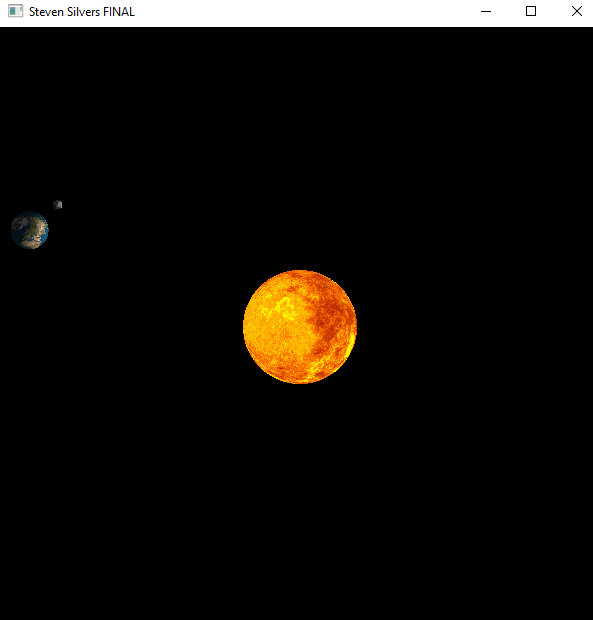
\includegraphics[scale=.5]{cap3}
		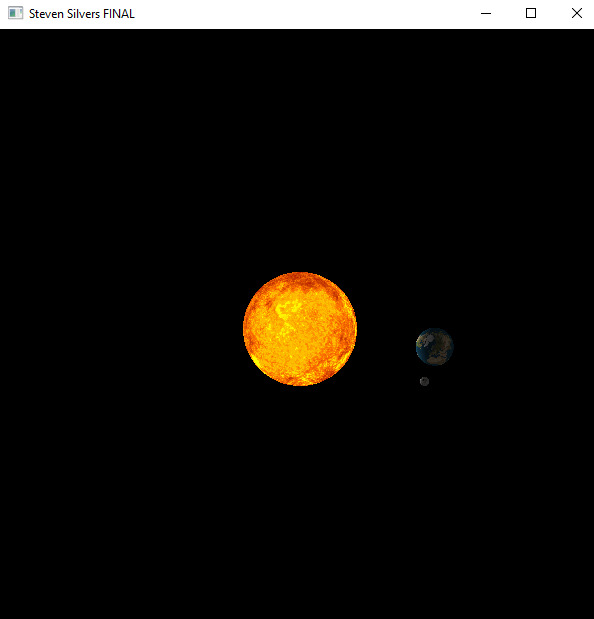
\includegraphics[scale=.5]{cap1}
		\caption{elliptical path of Earth}
	\end{figure}
			I elected not to put the moon on an elliptical path due to the exaggeration of distances in my simulation. Using a circular path for the Moon makes the interaction between the Moon and Earth easier to do and look less cluttered in the end.
	\newline
	\par
			The final step was to enable lighting and make the Sun a point light shining on the Earth and Moon. I achieved this by using the functions given in the lighting project earlier this term to create the light, with slight modification to add ambient light so that the dark sides of the Earth and Moon were still visible. I initially had trouble with the lighting because I forgot to modulate the textures, so no matter what I tried with altering my point light the change in lighting was still not reflected in the textured objects of the system.
	
	
	\begin{figure}[h]
		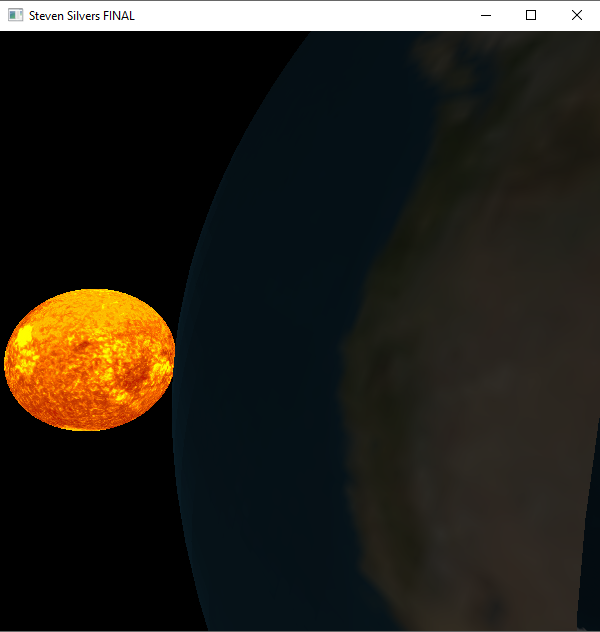
\includegraphics[scale=.67]{cap2}
		\caption{Watching the Sun set from Oregon viewpoint}
	\end{figure}

\end{document}